\chapter{Introdução}

O interesse da população pela robótica educacional vem aumentando nas últimas décadas oferecendo benefícios em todos os níveis da educação, seja no ensino de crianças, adolescentes ou adultos \cite{alimisis}. Um outro aspecto observado na literatura é que muitas aplicações de robótica são utilizadas para ajudar no aprendizado da matemática, ciência ou engenharia através de atividades práticas que envolvem a programação de robôs \cite{Benitti2012}. A programação de robôs educacionais oferece apoio para o ensino e aprendizagem de programação, principalmente para aqueles que estão iniciando a construção do pensamento computacional, com o propósito de usar o raciocínio lógico para estruturar soluções coerentes para problemas complexos \cite{Bombasar2015}.

Ambientes de programação de robôs são utilizados para a criação de atividades com este fim, onde os ambientes são geralmente atrativos e lúdicos, assim pode despertar o fascínio e a curiosidade dos estudantes pela programação (SILVA et. al, 2014). Segundo o jornal Folha de Pernambuco (2016), o recente do uso desses ambientes de robótica na sala de aula como forma de apoio nas escolas públicas do estado de Pernambuco tem aumentado o interesse dos estudantes pelas disciplinas de matemática e física, ainda afirma que o uso efetivo da robótica educacional aumenta a criatividade, sociabilidade, a concentração e o senso de coletividade.

O ambiente de programação para o LEGO MindStorms é um exemplo de aplicação com essa finalidade; apresenta uma interface para que o aluno possa escrever seus programas e executar o programa em robôs educacionais. Um problema no uso da robótica educacional é o alto custo para adquirir equipamentos, como por exemplo, o robô MindStorms da LEGO. Uma alternativa para o uso de robôs é utilizar ambientes de robótica educacional baseados em simulação como o RoboMind. Estes ambientes permitem a simulação passo a passo do robô, a partir da execução dos comandos do programa, ocasionando em uma melhor compreensão para o aluno (LESSA et al., 2015). 

Um problema dos ambientes de simulação de robôs é que estes não oferecem um mecanismo de verificação automática das soluções propostas por estudantes, ou seja, os programas escritos pelos alunos não são verificados quanto a sua corretude para o problema proposto, de modo que estudante e professor possam obter feedback automático sobre o funcionamento dos programas. O atual mecanismo de verificação em ambientes de simulação de robôs virtuais ocorre através da observação dos passos do robô, o que pode tornar uma tarefa demorada e trabalhosa. Além de onerosa, a verificação pode ser complexa. Por isso, métodos de verificação automática são tão importantes para determinar a corretude de um programa em diferentes perspectivas de maneira automatizada e rápida \cite{Duarte}. 

Portanto, este trabalho propõe uma abordagem para a tradução automática de uma linguagem de programação de robôs para um modelo formal com o objetivo de fornecer a alunos e professores uma forma de apoio durante a programação nesses ambientes por meio de feedback automático. Além disso, este trabalho contribui para a área da Engenharia de Software através da junção da educação com a verificação de sistemas de software, por meio da abordagem proposta para resolver o problema descrito em seguida


\section{Problema de Pesquisa}
Não existem ambientes gratuitos de programação de robôs que oferecem a estudantes e professores um mecanismo de análise automática dos programas. O único ambiente de verificação para robôs é o Robomind Academy\footnote{https://www.robomindacademy.com/}. Este ambiente além de ser pago, só permite a verificação dos mapas já cadastrados no sistema, que estão associados a desafios de programação fixados; não é possível realizar a verificação automática dos programas levando em consideração diferentes mapas e soluções para um determinado problema. Exemplos de problemas são: identificar se o robô encontra a saída de um labirinto; se o robô encontra um objeto no mapa; ou simplesmente se o robô termina sua execução (não executa um laço infinito).

%O RoboMind, mostrado na Figura \ref{fig:robomind}, é um ambiente de programação de robôs virtuais para o ensino e aprendizagem de robótica; possui uma interface com um espaço para a escrita dos programas e um outro espaço onde o aluno pode acompanhar a execução do robô em um mapa. Nesse ambiente, os programas são escritos na linguagem ROBO, uma linguagem educacional desenvolvida para a programação de robôs que oferece os principais comandos de programação: estruturas condicionais, estruturas de repetição, procedimentos e declaração de variáveis. O programa ROBO, ilustrado no lado esquerdo da Figura 1, movimenta o robô enquanto o objeto (beacon) não é detectado à sua frente: se não há nenhum obstáculo à sua frente, o robô avança uma célula (forward), caso contrário o robô recua uma célula (backward) e muda sua orientação para a direita (right).


O presente trabalho propõe a verificação automática de robôs programados na linguagem ROBO considerando diferentes mapas e desafios utilizando a técnica de verificação de modelos. Os programas considerados em ROBO possuem uma quantidade finita de estados, portanto a técnica possibilita realizar análises completas neste contexto.

Um dos problemas para realizar verificação de modelos é que não existe modelo formal para linguagens de programação de robôs. Um trabalho anterior (NOGUEIRA et. al, 2016) propõe a sistematização do processo de tradução dos programas escritos em ROBO para um modelo formal.  Neste trabalho é utilizado a verificação de modelos para automatizar a verificação de programas de robôs virtuais no ambiente RoboMind. Sua abordagem de verificação se dá por meio de algumas etapas como mostrado na Figura 2. É usado como entrada o programa escrito na linguagem ROBO e o mapa no qual o programa será executado. Através de um processo de tradução manual (baseado em um conjunto de regras de tradução), é obtido como saída a especificação formal do programa. Através de um processo automático é obtida a representação formal do mapa. A especificação formal do mapa e do robô são entradas do verificador de modelos para verificar as propriedades do robô. Como exemplo de propriedade, temos se o programa possui deadlock, ou seja, se o programa termina sua execução. 

\begin{figure}[h]
\centering
\caption{Visão geral da abordagem de verificação automática}
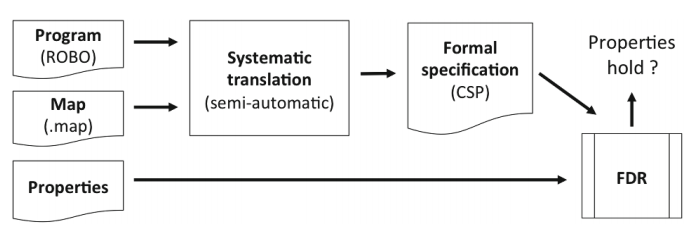
\includegraphics[height=5cm]{figuras/approach_workflow.png}
\fonte{\cite{nogueira}}
\label{fig:fluxograma}
\end{figure} 

Em \cite{nogueira}, a especificação formal (ou modelo formal) é construída na linguagem de álgebra de processos CSP (\textit{Communicatting Sequential Processes}). CSP é uma ótima linguagem para expressar também a execução simultânea de vários robôs em um mesmo programa. Tal possibilidade não foi explorada por trabalhos disponíveis na literatura.

A maior complexidade da abordagem ilustrada na Figura 2 é a tradução da notação ROBO para a notação formal. Esta tradução requer a definição de regras de mapeamento de cada elemento da linguagem ROBO para o seu equivalente em CSP, além da implementação de um compilador que automatize a aplicação das regras. No processo de criação do compilador, primeiro, as regras de mapeamento devem ser realizadas utilizando um framework que comtemple as etapas de criação de uma Linguagem de Domínio Específico (Domain-Specific Language - DSL). As DSLs são linguagens de alto poder de abstração linguístico onde o desenvolvedor pode focar na lógica da aplicação, o que permite que elas possam ser automatizadas, analisadas e otimizadas. As etapas fundamentais para a criação de uma linguagem de domínio específico são: (1) criar um parser para a sintaxe da linguagem; (2) desenvolver a análise semântica para a validação; (3) manipular programas de DSL por meio das transformações; (4) realizar a geração de código executável; (5) integrar a linguagem dentro de um ambiente de desenvolvimento (LENNART; KATS, 2010). No contexto deste trabalho, a DSL corresponde a linguagem ROBO. Para esta DSL, a compilação deve considerar toda a sintaxe da linguagem ROBO, desde comandos padrões (condicionais e repetição) até mesmo declaração de variáveis e procedimentos. Para esta pesquisa o framework Spoofax, o mesmo mostrado no artigo anterior, é adotado para realizar o mapeamento de ROBO para CSP, pois oferece um ambiente de desenvolvimento completo durante as etapas de criação de uma DSL.

Atualmente, o compilador de ROBO para CSP não considera vários elementos importantes da linguagem como variáveis e procedimentos. Além disto, não existe uma integração do compilador com o FDR. Também não existe uma interface que permita ao usuário utilizar a abordagem da Figura \ref{fig:fluxograma} de forma transparente. Desta forma, o problema que este projeto se propõe a resolver é:
Como especificar regras de mapeamento de ROBO para CSP usando o framework Spoofax para programas que incluem variáveis e procedimentos para que seja integrado, juntamente com o verificador de modelos FDR, em a uma única ferramenta de forma transparente para o usuário do RoboMind?

\section{Objetivos}
Nesta seção estão dispostos os objetivos pretendidos por esta pesquisa.
\subsection{Objetivo Geral}

O trabalho proposto tem como objetivo a extensão e a automação de uma abordagem de tradução de uma linguagem através do desenvolvimento de um compilador com finalidade de realizar verificação automática de programas de robôs educacionais por meio de um modelo formal.

\subsection{Objetivos Específicos}

\begin{enumerate}
    \item Definir regras de compilação para variáveis e procedimentos;
    \item Estender o compilador existente da linguagem de programação ROBO para notação formal CSP;
    \item Propor um protótipo funcional para análise de programas que integra o compilador com o verificador de modelos definido para este projeto.

\end{enumerate}

\section{Organização do Trabalho}